% This is the LaTex template file for the Journal "Language Development Research"
% Version: 1.0 (2022)
% Author: Mitja Nikolaus (mitja.nikolaus@posteo.de)
% Compile this file using pdflatex.
% The repository for the source files can be found at
%
%     https://github.com/mitjanikolaus/ldr-template
%

\documentclass{ldr-article}
\usepackage{easyReview} % for \comment, \alert, etc.
\usepackage{biblatex}
\usepackage{authblk}
\usepackage[shortlabels]{enumitem}
\addbibresource{main.bib}

% here we can set the page counter to the correct global page counter
\setcounter{page}{1}

% Here we can set the correct volume and issue number for accepted articles
\fancyfoot[C]{\titlepagefontsize Volume X, Issue Y, 23 June 2023}


\title{A proof-of-concept process for validated brain emulation boot-strapped on an in-silico fully known ground-truth neural circuit}

\author[1]{Randal A. Koene}
\author[1]{Thomas Liao}
\affil[1]{Carboncopies Foundation for Brain Research}

%\date{}                     %% if you don't need date to appear

\def\firstexp{\textit{e0\_bs} }

\begin{document}

    \maketitle

    \begin{abstract}
       \alert{REWRITE}: 
       There is presently not a single published proof-of-concept example where a process of brain emulation has been carried out at some scale and where a validation was performed to quantify the degree to which an emulation satisfies necessary success criteria. Scientific motivation to make progress in brain emulation depends on having a touch-stone implementation and reference evaluation to quantitatively improve upon. The only way to evaluate claims of brain emulation is through the use of metrics that compare an emulation with an original system. Similarity metrics must measure similarity in ways that matter to the goal of whole brain emulation, i.e. that satisfy cognitive success criteria. E.g. spike train timing is not duplicated, but the probability of spiking is modulated sensibly and the evolution of system attractors is plausible. Similarity metrics are needed at multiple levels and while some can be used only with fully known ground-truth systems, others will carry over to whole brain systems. The principle of brain emulation depends on the ability to satisfy cognitive success criteria while replacing implementation details at some scale. In analog, potentially chaotic systems, scale separation is achieved through the application of operational constraints. E.g. rhythms (brain) or clock cycles (computer), neural population activity (brain) or parity bits (computer), action potentials (brain) or binary thresholds (computer). The application of constraints at consecutive levels limits the size of each black box in system identification.
    \end{abstract}
    
    \keywords{brain emulation; system identification; similarity metrics; in-silico}
    \correspondingauthor{Randal A. Koene, CSO, Carboncopies Foundation for Brain Research, Sacramento, CA, Email: rkoene@carboncopies.org.}
    \orcids{https://orcid.org/0000-1234-5678-9999; }
    % for multiple ORCIDs, use \orcids and URLs separated by semicolons, e.g.:
    %\orcids{https://orcid.org/0000-1234-5678-9999;https://orcid.org/0000-5678-1234-9999}
   % \citationinfo{Other, A.N., Kramer, W.K., \& Pierce, J. (2022). Article title goes here. \textit{Language Development Research, 2}(1), XX–XX. \url{https://doi.org/10.34xxx/xxxx-xxxx}}


% =================================================================================
% SECTIONS PART 1 - problem description (paradigm change and translation challenge)
% =================================================================================

\section{Introduction}

With the availability of high throughput electron microscopy, exapansion microscopy, Calcium and voltage imaging, co-registered combinations of these techniques~\cite{phelps2021,court2023} and further advancements, high resolution data sets that span multiple brain regions or entire small animal brains such as Drosophila~\cite{zheng2018} may now offer inroads to expansive neuronal circuit analysis~\cite{scheffer2020,buhmann2021}. Results of such analysis represent a paradigm change in the conduct of neuroscience. So far, almost all investigations in neuroscience have relied on correlational studies, in which a modicum of insight gleaned from observational data leads to the formulation of mechanistic hypotheses, corresponding computaitonal modeling, predictions made using those models, so that experimental testing of the predictions offers support or modification of hypotheses. These are indirect methods for the study of a black box system of highly complex internal structure, recently critiqued as being unlikely to lead to a full understanding of brain function~\cite{jonas2017}. Large scale, high resolution reconstruction of brain circuitry can instead lead to mechanistic explanations and predictions of cognitive function with meaningful descriptions of representations and their transformation along the full trajectory of stages in neural processing. Insights that come from circuit reconstructions of this kind, a reverse enginering of cognitive processes, will lead to valuable advances in neuroprosthetic medicine, understanding of the causes and effects of neurodegenerative disease, possible implementations of similar processes in artificial intelligence, and in-silico emulations of brain function.

\alert{REWRITE}: A description of the aim of reducing the abstraction level and increasing the resolution at which modeling takes place until computational reconstructions have the functional characteristics of a specific sample, animal or person.

These aims include not just correlational predictions, but a complete mapping that describes how representations have ``meaning'' from step to step within the propagating activity of a system. And these aims include identifying subjective uniqueness, and being able to recreate that in prosthetic form. A neuroscience of reconstruction must emphasize not just shared operational fundamentals but individually unique functional structure, such as that which enables retrieval of animal-specific or personal memories.

The modeling process for the detailed reconstruction of specimen-specific neural circuitry is, at high resolution (neuronal morphology, synapse placement, ion channel characteristics) carried out using well known computational modeling techniques. Patch-clamp studies of synaptic and neural response, interactions along stretches of dendrite, application of algorithmic models that characterize dynamic behavior of ion channels produce predictive computational models at this resolution~\cite{markram2015}. 

Dynamic behavior at this resolution is stochastically characterized and easily influenced by small parameter changes, such as result from uncertainties in collected brain data or reconstruction errors. Large scale circuits composed of these high resolution models could exhibit divergent behavior of a chaotic nature due to such dependencies unless well constrained at a higher level of abstraction. This is the level of complex systems with emergent properties. That such constraints must be involved with reliable brain function is clear, given the remarkable robustness of cognitive function that depends on reliably cooperating activity in multiple brain regions under widely varying circumstances. A number of homeostatic or error correcting constraints have already been identified in theory and in practice. They include a reliance on neuronal population activity, transmission through groups of synapses, propagation through spikes and bursts, the applicaiton of lateral inhibition, phase locking by global modulating rhythms, and much more. A sensible application of constraints at successive levels of a detailed functional reconstruction will be essential.

\alert{REWRITE}:
The problem of satisfactory derivation of model parameters from data, identification and application of constraints is unsolved, building specimen-specific large scale neural reconstructions is relatively new, although reconstruction of individual neurons has history (e.g. see BlueBrain papers).

\alert{REWRITE}:
The problem has similarities with those in AI, where complex features and behaviors expressed in real world data need to be captured in rigorous and validated algorithms.

At present, there is no published proof-of-concept procedure by which to reconstruct, emulate and validate the circuit function of sample brain tissue at a scale that includes short- and long-distance connections contained in recent electronmicroscopy connectome data. In fact, the success criteria to which validation and verification of such emulation belong have not been established. 

Efficient improvement of methods is possible with rigorous testing, applying metrics when it is possible to determine errors precisely by comparing results achieved with intended correct results. This is possible when the original neural system examined is known fully. Such a system provides a ground-truth to strive for. Validation metrics derived from success criteria will measure similarities and deviations that matter to the cognitive functions of a (whole) brain emulation. For example, although a spatio-temporal pattern of spikes is rarely, if ever, duplicated precisely in neurobiological systems, sufficient approximation of spike probabliity as a function of time is a relevant measure.

\alert{REWRITE}:
Similarity metrics must measure similarity in ways that matter to the goal of whole brain emulation, i.e. that satisfy cognitive success criteria. E.g. spike train timing is not duplicated, but the probability of spiking is modulated sensibly and the evolution of system attractors is plausible. Similarity metrics are needed at multiple levels and while some can be used only with fully known ground-truth systems, others will carry over to whole brain systems. The principle of brain emulation depends on the ability to satisfy cognitive success criteria while replacing implementation details at some scale. In analog, potentially chaotic systems, scale separation is achieved through the application of operational constraints. E.g. rhythms (brain) or clock cycles (computer), neural population activity (brain) or parity bits (computer), action potentials (brain) or binary thresholds (computer). The application of constraints at consecutive levels limits the size of each black box in system identification.

% =================================================================================
% SECTIONS PART 2 - introduction to the data (e.g. the process that leads to the data)
% =================================================================================

\subsection{From brain matter to stacks of image data}

\comment{The first and foundational milestone for feasible whole brain emulation is an ability to acquire complete high resolution data from nervous systems up to the scale of the human brain.}{This only talks about the data as obtained via EM imaging, even though the challenge can also provide functional data. That may be okay, as this is still the part of the paper discussing the problem. Alternatively, we could be more general in our problem description.}

\alert{REWRITE:} There are now nanoscale morphology and connectome data sets available from a single sample for complete Drosophila brain and for multiple cubic millimeters of mouse brain.

\alert{REWRITE:} A new project has already been launched to obtain such a data set for an entire mouse brain.

\alert{REWRITE:} These are data sets that contain high resolution details for many connected brain regions, short- and long-distance connections in complete neural circuits.

\alert{REWRITE:} Identifiable features that correspond to specific neuron types, and more.

\alert{REWRITE:} There is a fair chance - if we knew what we were doing in terms of translation to model architecture and parameters and in terms of constraints and error correction - that existing data is enough to produce a working functional reconstruction of the fruit fly brain.

\subsection{From images to traced 3D objects}

\alert{REWRITE:} Advanced sample preparation and microscopy technology – using electron microscopes and, sometimes coregistered, light microscopes – were used to obtain stacks of images.

\alert{REWRITE:} Those are then stitched together and reconstructed to form a 3D visual representation consisting of high resolution voxels that measure mere nanometers on each side.

\alert{REWRITE:} Automated tracing algorithms, such as those developed at Google, are able to show the detailed morphology of neural cell bodies, axons, dendrites, synaptic spines, postsynaptic densities, glial cells, vasculature throughout a 3D reconstruction.

\alert{REWRITE:} This takes us from voxels to 3D objects, the first step in data processing, much as one might go from individual 1 ms voltage measurements to a voltage trace over time when the data collection instrument is an electrode, or from snapshots of luminescence to voltage traces over time when the data collection instrument is Calcium imaging.


% =================================================================================
% SECTIONS PART 3 - state of the art (many ideas, little validation/verification)
% =================================================================================

\section{Translation from brain data to model parameters}

\alert{REWRITE:} The goal is to reconstruct the working cells and neural circuits, able to process information and reproduce the cognitive behavior of the brain that was scanned.

\alert{REWRITE:} Translating measurable, observable data to correct model architecture of functional model parameters is now the primary scientific challenge.

\alert{REWRITE:} We had gone from voxels to 3D objects. Now we need to go from 3D objects to interacting sets of equations.

\alert{REWRITE:} A small number of leading research groups are reconfiguring their efforts towards this goal in a way that will obviously be paradigm changing in neuroscience.

\alert{REWRITE:} And some different methods are being tried.

\alert{REWRITE:} One is to measure components and to derive from that likely electrical properties.

\alert{REWRITE:} Another is to train machine learning to recognize features by having coregistered Calcium imaging with structural scans.

\alert{REWRITE:} Then there is the putative use of tags that could identify components by unique proteins.

\alert{REWRITE:} And in some cases, advances are attempted by using a rough identification of principal cells and interneurons to make circuit predictions (Shiu et al).

\comment{ADD LIST OF PAPERS WITH CANDIDATE METHODS, FIRST POSSIBLE CONTESTANT:}{The idea here is that we already identify some of those who we hope will take the challenge and call them out. We may then take one or more of these and attempt them on our ground-truth systems ourselves as a demonstration.}
\begin{itemize}
	\item add here...
	\item and more...
\end{itemize}


% =================================================================================
% SECTIONS PART 4 - proposing a solution (how validation and accelerating iterative improvement, competition of methods, are achieved in other domains)
% =================================================================================

\section{Validation, verification and competitive improvement}

\alert{REWRITE:} In machine learning and artificial intelligence, it is understood that successfully training a system requires not just a training data set but also validation and verification stages, a way to measure the performance of the system.

\alert{REWRITE:} Standardized, well-understood challenges

\alert{REWRITE:} AI algorithms → tested / compared on well known standard test sets (e.g. ImageNet)

\alert{REWRITE:} Well understood data sets, tuned to aims and requirement → thorough, fair, rapid feedback → rapid growth of neural reconstruction



\alert{REWRITE:} Similarly, the performance of a resulting emulation, created using a candidate reconstruction procedure that includes system identification and translation of data to parameters needs to be testable.

\alert{REWRITE:} Without that, it is impossible to make claims about the correctness of the outcome or to compare different methods.

\alert{REWRITE:} Some metrics have been applied in functional neuroprosthetic methods, such as work by Dong Song and others on the hippocampal prosthesis, where the I/O of the emulation must match an envelope around recorded activity.

\alert{REWRITE:} Here we run into a problem for structure to function translation.

\alert{REWRITE:} No one knows what the circuits inside a Drosophila brain or a mouse brain are supposed to be. So, how do we know if the ones we reconstructed are right or wrong? How wrong? And where are the mistakes to correct?

\alert{REWRITE:} Sure, we have some idea of the external behavior of a fruit fly or a mouse. If the model is of a whole brain and the emulated animal runs at all and can still find its way through a maze then you’re probably fine. But that is incredibly unlikely in early models.

\alert{REWRITE:} More likely, the model does not run, or it runs, but produces no recognizable behavior. Then what?

\alert{REWRITE:} One cannot tell if there are hidden errors that produce a problematic evolution of the behavior of the reconstructed animal, errors that did not manifest in the experimental condition tested.

\alert{REWRITE:} Imagine that you were trying to reverse engineer and reconstruct a microchip, but you have no idea what the full set of I/O functions of the original chip are supposed to be. Worse, you may not even understand that it is using a binary code, that a specific number of channels together form symbols. If you then look at the microchip under a microscope and you use some method to convert what you see into conductivity equations, how would you know where to look for mistakes when it misbehaves?

\alert{REWRITE:} Develop serialized, standardized whole-brain emulation challenge (platforms: VBP + NES) - rigorous, trusted

In the fields of machine learning and artificial intelligence, it is commonplace that new algorithms are tested, compared, and prove themselves through their performance on well understood standardized data sets, such as ImageNet~\cite{deng2009,russakovsky2015} and others. The nascent field of neural system reconstruction or brain emulation will grow rapidly through fair, thorough and rapid feedback as soon as there are solid and well understood challenge data sets, well tuned to aims and requirements.

\alert{REWRITE:} This is something that an objective, rigorous and trusted neutral party, a team working at the Carboncopies Foundation can provide.

\alert{REWRITE:} Therefore, we decided that the first end-to-end project for our BrainGenix-NES and Virtual Brain Platforms is to develop a serialized and standardized whole-brain emulation challenge.

\subsection{Applying validation metrics: Structure}

Identifying the cell bodies of neurons in high-resolution 3D reconstructions of microscopy data is relatively easy and not very error prone. For this reason, although validation will confirm neurons found, the point cloud that is composed of identified neuron centers provides fairly reliable information with which to to align a proposed emulation with the ground-truth. A neuron to neuron mapping results. Once emulation neurons are mapped to ground-truth neurons, there are many ways to validate structure and function of the whole network, as well as more manageable smaller sub-circuits, without immediately running into the curse of dimensionality.

\subsubsection{3D alignment of point clouds}

\subsubsection{Validating structure at the individual neuron level}

\subsubsection{Validating structure of sub-circuits}

\subsubsection{Validating structure of the whole network}

\subsection{Applying validation metrics: Function}



% =================================================================================
% SECTIONS PART 5 - implementing the solution (competition on known ground-truth systems, WBE challenge, two essential components: 1 - success criteria expressed by validation metrics, 2 - fully known ground-truth systems needed for rigorous metrics and performance)
% =================================================================================

\section{The challenge: Competing on fully known ground-truth systems}

\alert{REWRITE:} There are two essential components: 1 - success criteria expressed by validation metrics, 2 - fully known ground-truth systems needed for rigorous metrics and performance).

\subsection{Fully known ground-truth systems}

\alert{REWRITE:} We provide brain data that was obtained from little brains, neural systems, for which we have the fully known ground-truth.

\alert{REWRITE:} Obviously, these fully known ground-truth systems cannot be fruit flies, mice, or even the nematode C.Elegans. After all, we actually need to know and understand the circuits within them.

\alert{REWRITE:} These are systems we have to create, and they come in two fundamentally different forms: In-silico and in-vitro.

\alert{REWRITE:} In-vitro, we grow neural cell cultures on top of electrode arrays.

\alert{REWRITE:} Their structure and connectivity is viewable under a microscope.

\alert{REWRITE:} The electrodes permit recording and stimulation of each neuron.

\alert{REWRITE:} The system is fully knowable in functional terms.

\alert{REWRITE:} In-silico, we develop simulated neuronal systems that give us even more degrees of freedom, precision control, testability and insight. Very useful for gradual increase of sophistication (see ladder of serialized challenges).

\subsection{Rigorous performance evaluation: Success criteria and validation metrics}

\alert{REWRITE:} A model presents an ideal, excluding some aspects of reality while including others, focusing on success criteria.

\alert{REWRITE:} Emulation objectives were used to formulate success criteria for an emulation.

\alert{REWRITE:} Success criteria lead to corresponding validation metrics that are applied.

\alert{REWRITE:} We started with 80 success criteria that were reduced by categorization into 25 significant to WBE.

\alert{REWRITE:} From these we extract 8 initial success criteria applicable to small neural circuit reconstructions. We are building validation metrics for these.

\alert{REWRITE:} The challenge participant receives a score on each and detailed feedback about system functions found, missed or confabulated, and about the location and type of errors, which hopefully help to further improve methods.

\alert{REWRITE:} WBE objectives → Success Criteria
80 → 25 (cat.) → 8 initial
Validation metrics
Score + Feedback

\begin{figure}
	\centering
	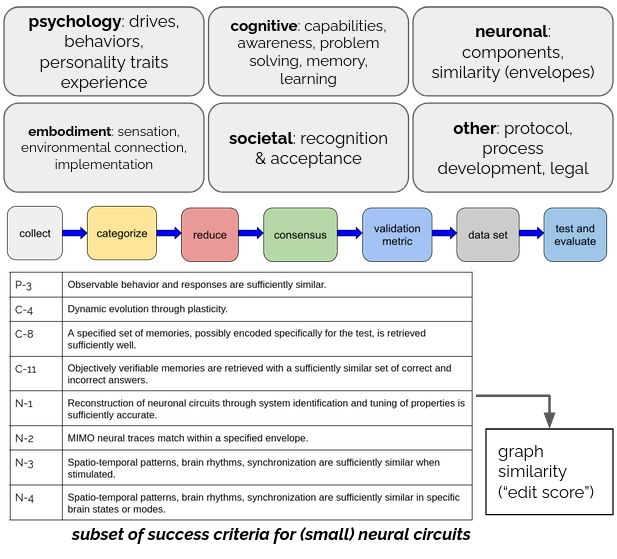
\includegraphics[width=1\linewidth]{figures/success-criteria.jpg}
	\caption{Success-criteria.}
	\label{fig:success-criteria}
\end{figure}


% =================================================================================
% SECTIONS PART 6 - the challenge taking process (with example)
% =================================================================================

\section{Taking the challenge}

\alert{REWRITE:} A challenge participant proposes a new method that assumes that data was acquired in some particular way. For example, the participant may require co-registered Calcium imaging.

\alert{REWRITE:} Because data acquisition requirements can be very specific (especially these early days) the team has to actively maintain the challenge, working with participants to provide the sort and format of data expected.

\alert{REWRITE:} The desired data acquisition approach is described to the whole-brian emulation challenge administering team. Physics applied. (See related work~\cite{aberra2018}.)

\alert{REWRITE:} The team has or creates a set of fully known ground-truth systems.

\alert{REWRITE:} The challenge admin team has a God’s Eye view of the system structure and function, and produces sets of acquired brain data. The ground-truth systems are not shared with the challenge participants. The participants receive the acquired data stack.

\alert{REWRITE:} The participants then apply their proposed methods and reconstruct one or more candidate emulated systems.

\alert{REWRITE:} The challenge admin team then compares the structure and performance of each emulated system side by side with the corresponding ground-truth system.

\begin{figure}
	\centering
	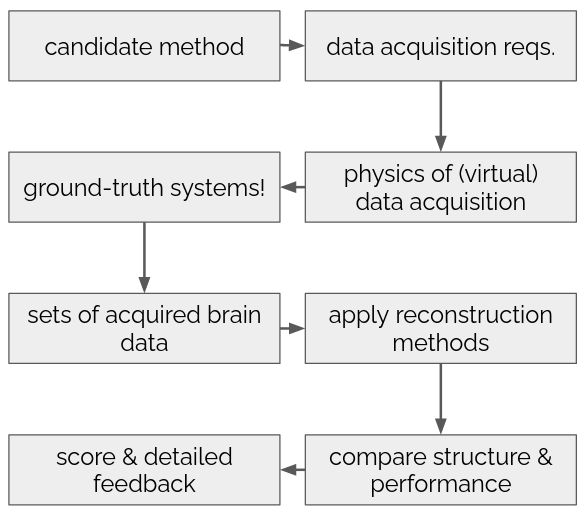
\includegraphics[width=1\linewidth]{figures/challenge-process.jpg}
	\caption{Diagram of the challenge process.}
	\label{fig:challenge-process}
\end{figure}

\begin{enumerate}
	\item Participant proposes method and expected data acquisition
	\item Admin team works with participant, physical sim of data acquisition
	\item Admin team has fully known ground-truth systems
	\item God’s Eye view of structure and function → data set produced for participant
	\item Participants apply methods → produce emulation
	\item Admin team compares ground-truth and emulation side-by-side
\end{enumerate}

\subsection{End-to-end example}

\comment{PROPOSED MODELING FOR US}{We can work our way up to what we want to show in the paper, for example, by doing the following sequence of things: (1) Raw and basic demonstration of the process by creating a ground-truth system, making an emulation by copying that with a few error-edits, applying metrics and presenting the result, (2) Attempting to apply published reconstruction methods on data ourselves to create an emulation, presenting results, (3) Improving our platform until that presentation with a published method works. To make this more fun, I popose that the ground-truth system we create should have a built-in cognitive function that does something, so that we can "discover" it.}

The ball-and-stick example is intended to provide the simplest in-silico case with the smallest
number of variables to address while still demonstrating the full process and dependencies
chain for whole brain emulation (see Fig.~\ref{fig:dependencies-pyramid}). This is an opportunity to anchor the development of useful similarity metrics for brain emulation.

In the following sections, we describe the process (parts I through XI) with the aid of an example experiment, \firstexp, that is designed as a simplest case in-silico with the minimum number of variables that can demonstrate the process. The abbreviation "bs" stands for ball-and-stick, because the neurons have only a spherical soma and a single axon component.

In-silico sample preparation (XI) and characterized physiology (IX and VII).
How we equate characterized ephys and biological brain samples with VBP architecture and components.

Establishing a set of virtual physiological components with well-characterized dynamics (requirement IX).

For the purposes of testing methods and metrics, within this virtual brain laboratory, we define both the \textbf{morphology} and \textbf{physiology} of virtual components that we declare to be our \textbf{ground-truth} about which we know everything. The components of the \firstexp ground-truth model are as follows:

\begin{itemize}
	\item The system comprises a set of brain regions.
	\item A brain region (\textit{BrainRegion}) has a specified geometric shape and specified physiological content in the form of neural circuits.
	\item The type of neural circuit defined in \firstexp is a linearly aligned ball-and-stick neural circuit (\textit{BS\_Aligned\_NC}), so called, because the morphology of the neurons is essentially a ball with a stick.
	\item A neural circuit consists of some number of cells. Each of the cells has a specified morphology, characteristic dynamic functions of the neuron, and connectivity established by specifying receptors between a pre- and post-synaptic cell.
\end{itemize}

In \firstexp, the morphology is specified as a spherical soma (\textit{BS\_Soma}) and a cylindrical axon (\textit{BS\_Axon}) of particular dimensions (Fig.~\ref{fig:KGT-architecture}). A location is specified on the morphology for each receptor (\textit{BS\_Receptor}).

\begin{figure}
	\centering
	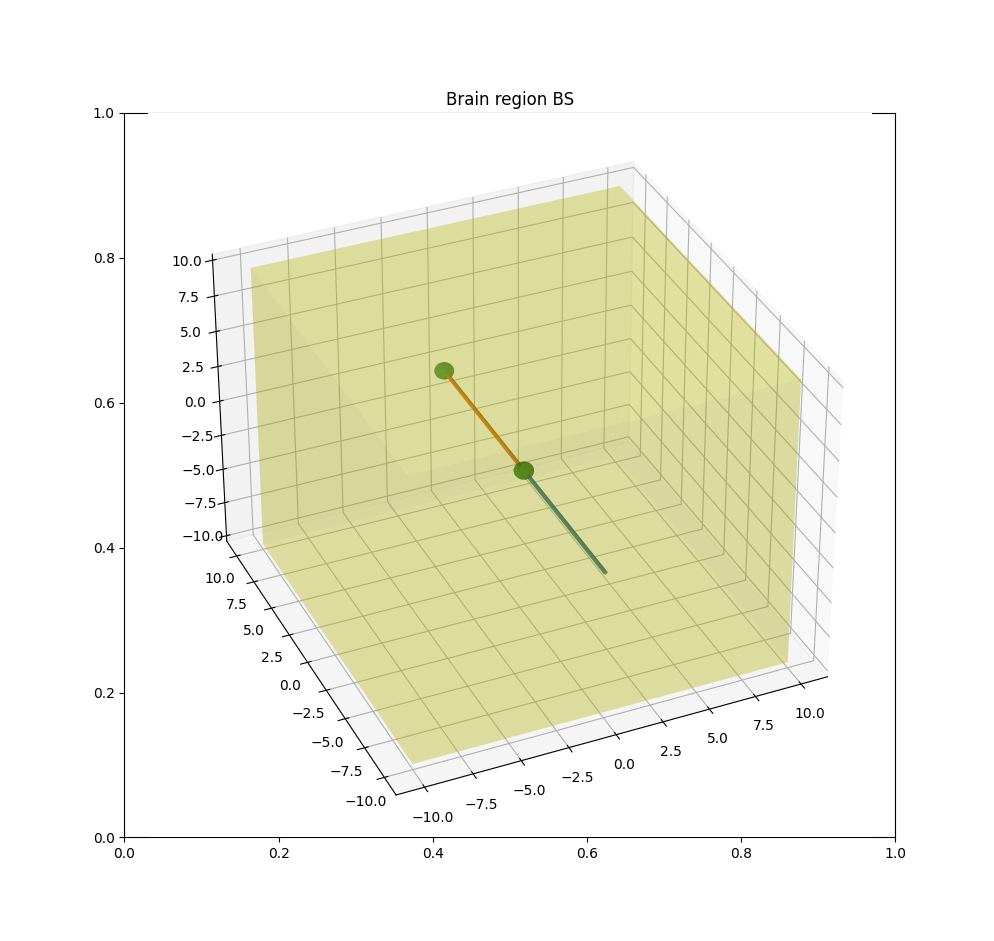
\includegraphics[width=1\linewidth]{figures/e0_bs.png}
	\caption{Diagram of the known ground-truth ball-and-stick neural circuit architecture within in-silico brain region.
	}
	\label{fig:KGT-architecture}
\end{figure}

Functional characteristics of each cell in \firstexp are specified by a neuron definition (\textit{BS\_Neuron}) and by weights associated with the synaptic receptors and their characteristic functions.

The \firstexp example is purposely extremely simple:
\begin{itemize}
	\item There is 1 brain region with a box shape, $20 \mu m$ on each side.
	\item The brain region contains a single neural circuit.
	\item That neural circuit has 2 neurons, one pre-synaptic, one post-synaptic.
	\item The neurons are identical, using the default parameter values for the ball-and-stick neuron class (\textit{BS\_Neuron}), see Table~\ref{tab:bs_neuron_default_pars}.
	\item The weight of the synaptic connection formed by a receptor has a value of $w_{syn} = 1.0$.
\end{itemize}

\begin{table}
	\begin{tabular}{ll}
		\centering
		Initial membrane potential & $V_m = -60 mV$ \\
		Resting membrane potential & $V_{rest} = -60 mV$ \\
		Action potential firing threshold & $V_{act} = -50 mV$ \\
		Spike potential during refractory period & $V_{spike} = 60 mV$ \\
		Time span of absolute refractory period & $\tau_{abs} = 1 ms$ \\
		After-hyperpolarization potential & $V_{AHP} = -20 mV$ \\
		After-hyperpolarization decay time constant & $\tau_{AHP} = 30 ms$ \\
		\hline
		Rise time constant of the post-synaptic potential & $\tau_{PSPr} = 5 ms$ \\
		Decay time constant of the post-synaptic potential & $\tau_{PSPd} = 25 ms$ \\
		Amplitude of the post-synaptic potential & $V_{PSP} = 20 mV$ \\
	\end{tabular}
	\caption{Default parameter values of ball-and-stick neuron class \textit{BS\_Neuron} and \textit{BS\_Receptor}.\label{tab:bs_neuron_default_pars}}
\end{table}

A simulation of activity in the ground-truth model carried out in small time increments (e.g. $1 ms$). For each neuron, the update function has two main steps:
\begin{enumerate}
	\item Update the momentary membrane potential, $V_m$.
	\item Detect threshold crossing and possibly generate a spike. This step is ignored if the neuron is still within the absolute refractory period, $\tau_{abs}$, of its most recent action potential.
\end{enumerate}

The momentary membrane potential is the sum of contributing potentials:
\begin{equation}\label{eq:membrane-potential}
	v_m(t) = V_{rest} + v_{spike}(t) + v_{AHP}(t) + \sum_i{v_{PSPi}(t)},
\end{equation}
where $v_{spike}(t) = V_{spike}$ during the absolute refractory period, and $v_{PSPi}(t)$ is the momentary post-synaptic potential contributed by the i-th receptor.

The refractory contribution of the spike:
\begin{eqnarray}
	v_{spike}(t) 	& = V_{spike} & \textrm{if } \Delta t_{act} \le \tau_{abs} \\
	& = 0 mV & \textrm{otherwise,} \nonumber
\end{eqnarray}
where $\Delta t_{act}$ is the time since onset of the most recent action potential.

Modulation of the membrane potential by after-hyperpolarization:
\begin{eqnarray}
	v_{AHP}(t)		& = V_{AHP} \exp(\frac{-\Delta t_{act}}{\tau_{AHP}}) & \textrm{if } \Delta t_{act} > \tau_{abs} \\
	& = 0 mV & \textrm{otherwise.} \nonumber
\end{eqnarray}

Post-synaptic contributions to the membrane potential caused by the propagation of pre-synaptic action potentials through input receptors:
\begin{eqnarray}
	v_{PSPi}(t)		& = w_{syn} V_{PSP} ( -\exp(\frac{-\Delta t_{act,i}}{\tau_{PSPr}}) + \exp(\frac{-\Delta t_{act,i}}{\tau_{PSPd}}) ) & \textrm{if the pre-synaptic neuron has spiked.} \\
	& = 0 mV & \textrm{otherwise,} \nonumber
\end{eqnarray}
where $\Delta t_{act,i}$ is the time since onset of the most recent action potential at the pre-synaptic neuron connected through receptor $i$.

A threshold crossing occurs if the new momentary membrane potential is at or beyond the firing threshold, $V_m \ge V_{act}$. If so, then a new spike onset time, $t_{act}$ is appended to the list of the neuron's spike times. That list is consulted by adjacent post-synaptic neurons that receive receptor input from this spiking neuron.s

In-silico representation of virtual brain components (requirement VII).
Describe preparation and use of the components library. Add reference to SW.

Preparation of the virtual brain architecture of the known ground-truth system (requirement XI).
Describe how the architecture is set up. Add reference to SW. I.e. describe the steps that the model script takes to get to a defined known ground-truth system.

\subsubsection{A virtual brain ground-truth system provides a ``God's eye'' record}

Every calculated variable can be recorded for analysis. That aids the development of similarity validation metrics.

\begin{figure}
	\centering
	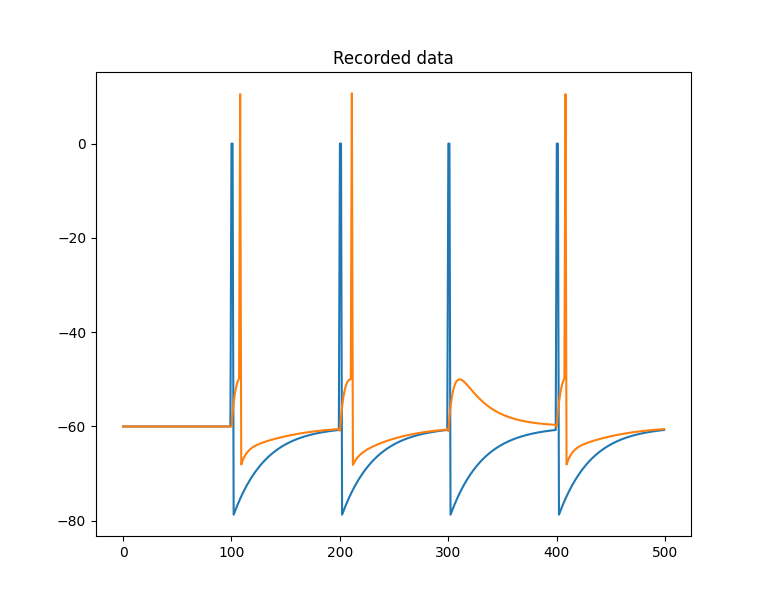
\includegraphics[width=1\linewidth]{figures/e0_bs_recorded.png}
	\caption{Plot of ball-and-stick neuron membrane potentials as recorded in ``God's eye'' mode during an experiment run.
	}
	\label{fig:ball-and-stick}
\end{figure}

This is not the same as the virtualized experimental data acquisition to be carried out in the origin system.

\subsection{Data acquisition: Double-blind experimentation in a virtual brain laboratory (requirements X and VIII)}

Even though the ground-truth model is fully known to the designer, the experimenter is blind to this and can use only data obtained through in-silico data acquisition that mirrors the process of data acquisition from biological brain systems.

Simulated data acquisition is not permitted the God's eye view. Instead, it is constrained to the use of simulated data recording devices and simulated stimulation devices.

Activity observed is the result of either spontaneous simulated activity in the ground-truth system or activity caused by simulated stimulation methods. These may be simulated stimulation electrodes, simulated optogenetic stimulation, or others.

Typical simulated functional data recording devices include simulated recording electrodes of various types, simulated calcium imaging in a number of variants, or even simulated fNIRS or fMRI. In each case, detectable contributions of neuronal activity are combined with confouding factors (including noise, unreliability, defects) in simulation of the physics involved in measurements.

Typical simulated structural data recording devices include simulated microscopy of various types (e.g. electronmicroscopy, two-photon, light-sheet, etc). Again, the resulting images combine information about the ground-truth system morphology with confounding factors and effects of the physics involved.

Simulated data acquisition can be sophisticated and can attempt to model realistic results closely. Alternatively, simulated data acquisition can purposely apply simplifications for the following reasons:
\begin{enumerate}
	\item Ease and rapidity of implementation.
	\item Reduced computational cost.
	\item Producing simplified laboratory condition examples with fewer variables to consider.
\end{enumerate}
The simplified laboratory conditions reason is particularly useful, because this allows methods to be tested first in vastly simplified conditions where the capabilities and limitations of the method can be identified, demonstrated and evaluated in their most obvious form, without distracting contributors.

\subsection{In-silico experimental data acquisition (requirement X)}

\alert{REWRITE:} Describe the data acquisition set up with the previously prepared KGT system and running data acquisition simulations. Add reference to SW.

The steps of simulated data acquisition are:
\begin{enumerate}
	\item Initialize the ground-truth model (loading or rerunning the previous stage).
	\item Initialize simulated functional data acquisition by placing simulated electrodes or by setting up simulated calcium imaging.
	\item Run simulated data acquisition and store that functional data.
	\item Run simulated imaging by obtaining 2D projections of the 3D model and store that structural data.
\end{enumerate}

\subsubsection{Initializing simulated functional data acquisition}

In our example experiment, \firstexp, preparation of simulated functional data acquisition involves these steps:
\begin{enumerate}
	\item Specify expected spontaneous activity of the neurons in the system.
	\item Set up a simulated single recording electrode in a location approximately between the two neurons.
	\item Set up a simulated calcium imaging microscope that sees both neurons.
\end{enumerate}

To specify the expected spontaneous activity, we pick a mean spontaneous firing interval, $280 ms$, and its standard deviation, $140 ms$. This will be the same for both neurons in the example system. We call the \textit{set\_spontaneous\_activity()} member function with a list that associates the mean-stdev pair with each of the enumerated neurons.

A call to the \textit{attach\_recording\_electrodes()} member function is used to set up any number of simulated electrodes. In our example, we provide a list with the specifications for only one electrode. We provide the following specifications:
\begin{itemize}
	\item The position of the tip of the electode, at the geometric center of the system.
	\item The positions of recording sites on the electrode, in this case one site at the very tip.
\end{itemize}

Similarly, a call to the \textit{attach\_calcium\_imaging()} member function is used to set up a calcium imaging device. In \firstexp, we specify:
\begin{itemize}
	\item Both neurons will fluoresce and show up during imaging.
	\item We will use a simulated jGCaMP8 calicium indicator~(\cite{zhang2023}) with relatively fast and short response dynamics, specified by an indicator rise time of $2 ms$ and an indicator interval of $20 ms$.
	\item The lens front position is $(0, 20, 0)$, $20 \mu m$ above the simulated sample, and is positioned vertically, as indicated by a rear position $(0, 40, 0)$.
\end{itemize}

\subsubsection{Simulating functional data acquisition}

Simulated electrode and calcium imaging devices record data while we run the model for a specified number of simulated milliseconds.

\alert{REWRITE:} more about how those simulated devices generate the recorded data by using simulated physics.


% Section about EM Rendering
\subsubsection{Simulating structural data acquisition}

We provide high-throughput microscope specifications:
\begin{itemize}
	\item Obtain images from the 'full' sample.
	\item The full sample is carved into sample sections $6 \mu m$ wide and long.
	\item Each image has $6000$ by $6000$ pixels.
	\item The voxel resolution (represented by each pixel) is $4 nm$ in x and y and $30 nm$ in the z dimension.
\end{itemize}

(Here: put more about how a simulated high-throughput EM image stack is generated using simulated optics.)

\begin{figure}
	\centering
	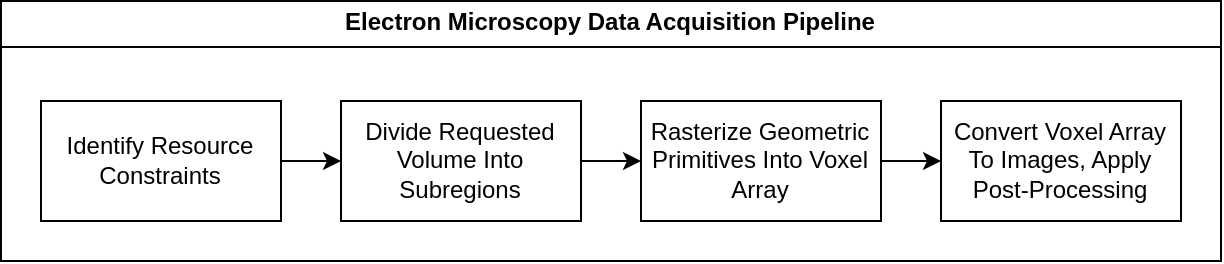
\includegraphics[width=1\linewidth]{Figures/VBP_EM_Render_Pipeline.drawio.png}
	\caption{High-level overview of the electron microscopy rendering process.}
	\label{fig:em-pipeline}
\end{figure}


Our approach involves three major steps. Firstly, we divide the volume into $n$ subregions, based on various system resource constraints. Next, we rasterize the geometric primitives used to represent the neural morphology in each subregion. Finally, the voxel array is traversed and converted to a 2D image array, post-processing applied, and saved.

% Todo: add detailed section describing each of these major steps
% Convert the above overview into a bullet-point based list
% Make a diagram showing the process? (maybe 3d, and have it show the voxel rasterization process? (better explainer than words))
% Also, describe some of the optimziations done and performance improvements
% Actually, the whole thing should be simplified a bit... (Don't include optimizations in the overview, add those in a subsection of this)
% right, that's all i think.



\subsection{Collected data and post-processing (requirement VIII)}

\alert{REWRITE:} Describe what it means for the collected data to be the "relevant" brain data.

\alert{REWRITE:} Describe the format of data obtained and how it may be post-processed for this simple experiment. Add reference to SW.

\subsection{Validation of candidate emulated systems using similarity and performance metrics based on success criteria for successful whole brain emulation (requirements I-III)}

\alert{REWRITE:} Describe similarity metrics that can be used in known ground-truth system and those that can be used in a broader category of systems, even biological brains. Explain that these will evolve as research proceeds from these most basic in-silico systems to more sophisticated systems.

\subsubsection{Measuring similarity and performance (requirement III)}

(Here: Describe the application of metrics and the evaluation of results.)

% =================================================================================
% SECTIONS PART 7 - results and how to use them
% =================================================================================

\section{Learning from performance and errors}

\subsection{Using known ground-truth systems to develop methods for the identification of error sources and their correction}

\alert{REWRITE:} Describe an example of an error and how its cause is determined. Describe how the system identification and translation is adjusted and the outcome improved. Add reference to SW.

\subsection{Meeting success criteria (requirement II)}

\alert{REWRITE:} Describe this important relationship.

\subsection{Achieving a successful whole brain emulation for the ball-and-stick neural system (requirement I)}

(Here: Describe the outcome.)

% =================================================================================
% SECTIONS PART 8 - progression (ladder of sophistication, in-silico to in-vitro to in-situ)
% =================================================================================

\section{A ladder of serialized challenges}

\alert{REWRITE:} The challenge is not a single challenge system. It is a serialized ladder of challenges.

\alert{REWRITE:} A challenger should begin by trying proposed methods with the easiest challenge, then work their way up the ladder.

\alert{REWRITE:} We can compare this with analogous challenges that have been used in the development of AI. For example, a first computer vision challenge might test the ability to distinguish clear images of bicycles from those of cars.

\alert{REWRITE:} Following computer vision challenges might add object rotations, occlusions, noise, etc.

\alert{REWRITE:} Challenges become progressively more realistic and progressively harder.

\alert{REWRITE:} We begin with very simple ground-truth systems that produce data sets much easier to interpret than real data sets.

This can be as simple as 2, 10, 20 or 100 “ball-and-stick” neurons, where the system morphology is restricted to spheres for cell bodies and single cylinders for axons. No other object in the interstitial spaces, no glial cells, no vasculature. Identification of components should be relatively easy at that stage.

More sophistication is added if the challenger is able to handle the simplified case. The next stage might have multiple neuron types, might have dendrites with detailed branching and functional effects of dendritic computation that depend on the locations of synapses.

At another stage, circuits may include recurrent connections.

Beyond that, we may require not merely static circuit reconstruction, but also correct emulation of plasticity functions, for success criteria that require that system behavior evolves within an acceptable envelope.

When you want to test if a student understands and can work with fundamental concepts you let them solve some problems with spherical objects in a vacuum, you don’t immediately ask for orbits involving realistic, oddly shaped bodies.

\alert{REWRITE:} Mention how one would proceed on to the next more sophisticated step and towards working with real brain tissue for which there is no known ground-truth.

\subsection{A level of ``minimal acceptable sophistication''}

As one considers reverse engineering a data stack from an example ground-truth system, for example, an IF-neuron implementation of XOR logic, it is clear that one needs to be able to distinguish types of neurons. Principal neurons with excitatory AMPA synapses to targets, as well as interneurons with inhibitory GABA synapses onto targets are both needed for that example. There are morphological characteristics that can be used to distinguish such neurons in reconstructions from EM data.

Simplifying, one might generate morphological representations in which all principal neurons have larger somas than interneurons, because human cortical principal cell somas typically have diameters of 10-50 um, while interneurons have diameters of 5-30 um. Allowing the overlapping diameters (10-30 um) introduces room for doubt during interpretation of morphology data.

At a more sophisticated level of representation, the presence of detailed dendritic arborization would provide additional clues in terms of characteristic shape, distribution of proximal and distal connections, and more, with which to identify reliably. So, while the simplified morphological representation is intended to present an easier entry point with fewer variables at which to test core competencies of reverse engineering methods, without additional known rules for that simplified universe there can be unintended new difficulties.

As with any simplified model of the world, such as a board game may be a simplification of a realistic battle, unintended uncertainties can be removed by providing additional in-universe ``rules''. For example, the overlapping diameter ranges could be disallowed. Or, EM data could include coloring that shows principal neurons in blue and interneurons in red. Alternatively, one might decide to skip levels of sophistication that lack characteristic detailing needed to avoid introducing new uncertainties, with a risk that the only levels detailed enough to provide all the clues needed for successful functional reconstruction are those as sophisticated as real-world data. Note competing considerations:

\begin{enumerate}[a)]
	\item Providing no unrealistic rules or expectations demands that challenge examples raise their detail level to the degree that provides all the clues needed to solve a specific example from its corresponding data stack. The onus is on the challenge developers to insure that this is so, with a potential downside that even the simplest examples are fairly sophisticated and contain a large number of variables. Resulting performance scores and identified error evaluations of submitted candidate emulations may be more complex, which might be a hurdle to iterative improvement at the early stages of developing a new system identification and translation method.
	
	\item At each level of sophistication, challenge examples come with a set of associated special rules (rules that are different than what we might expect in the real world). This means that a reverse engineering technique meant to be applied to real world data might need some adjustment to be applied to the example data stack. This might seem to give contestants more work to do. On the upside, this approach may permit better separtion and stepwise advancement along different dimensions of the core competencies of a suite of system identification and translation methods. For example, at the simplest level the data stack would not be intended to test the ability to identify a neuron type by its morphology, but instead would focus on a method's ability to capture the full graph structure of a system and to combine extracted system architecture with selections from a functional library.
\end{enumerate}

\subsection{Comparing performance across hypothetical domains of data distortion}

\alert{REWRITE:} There is a lot of concern in every connectomics method about distortions, shears, other issues in the sample, depending on the sample prep method used. Testing the same reconstruction method on data that has experienced zero to many such problems could be really informative about functional robustness and the degree to which reconstruction methods suffer. It's another dimension of the test space supplied to candidates. That doesn't just test reconstruction methods it also compares pros and cons of different sample prep and microscopy methods. I think this deserves its own section in the paper, just to introduce that part of the challenge. (And it's yet another thing other platforms do not provide.)

\subsection{Real-world conditions and animal brains}

At every level of sophistication, models and their components must have form (spatial definition) and function (activity definition). This ensures a link between structure and function, which realistic translation and system identification candidates will need to make use of.

Eventually, the sophistication of the in-silico ground-truth systems begins to approximate that of an in-vitro ground-truth system.

After successful validation with such systems the application of translation and system identification methods can proceed to partially knowable systems

E.g. slices of neural tissue.

E.g. tiny animals, such as the C.Elegans nematode (Kording Lab focus).

\begin{enumerate}
	\item form and function at each level of sophistication
	\item in-silico sophistication begins to approximate in-vitro
	\item proceed to partially knowable systems
	\item e.g. slices, tiny animals
\end{enumerate}

\begin{figure}
	\centering
	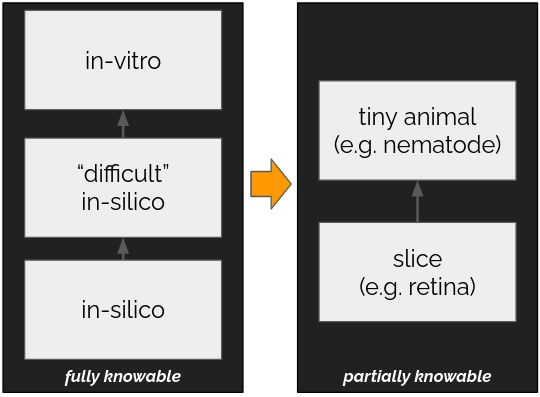
\includegraphics[width=1\linewidth]{figures/to-animal-brains.jpg}
	\caption{To animal brains.}
	\label{fig:to-animal-brains}
\end{figure}


\section{Discussion}


% Broken for now, disabling (due to same issue with biblatex, please fix dependencies Randal!)
\printbibliography

\section{Data, Code and Materials Availability Statement}

\alert{REWRITE:} Add links and DOIs to data, code and related materials.

\section{Authorship and Contributorship Statement}

\alert{REWRITE:} List who conceived the study, who designed the study and wrote the first draft of the manuscript. List other contributions. Mention if someone analysed data and revised the manuscript.

All authors approved the final version of the manuscript and agree to be accountable for all aspects of the work in ensuring that questions related to the accuracy or integrity of any part of the work are appropriately investigated and resolved.

\section{Acknowledgements}

\alert{REWRITE:} Add acknowledgments if applicable. This can include an acknowledgment of early support provided to the project.

\clearpage
\appendix

\section{Appendices etc.}

\alert{REWRITE:} Only if applicable.

\end{document}
